\section{Dữ liệu}
\label{sec:data}

\subsection{Mô tả tập MNIST}
MNIST %\cite{lecun1998}
gồm 70.000 ảnh xám $28\times28$ của các chữ số 0--9, chia sẵn thành 60.000 ảnh huấn luyện và 10.000 ảnh kiểm thử. Ảnh được tạo từ hai cơ sở dữ liệu của NIST (SD-3 do nhân viên Cục Điều tra Dân số Hoa Kỳ viết, SD-1 do học sinh trung học viết): mỗi chữ số được thu về khung $20\times20$ (giữ tỉ lệ, khử răng cưa) rồi đặt vào ảnh $28\times28$ sao cho khối tâm nét chữ trùng tâm ảnh. Người viết của hai tập không trùng nhau, nên tập kiểm thử đo được khả năng tổng quát hoá sang người viết mới.

Lớp \code{MNISTLoader} (\code{src/data.py}) tải bốn file gốc định dạng IDX. Mỗi file có phần đầu nhị phân big-endian chứa \emph{magic number} (2051 với ảnh, 2049 với nhãn), số mẫu và kích thước ảnh; chương trình kiểm tra các trường này cùng miền giá trị nhãn trước khi lưu thành \code{data/mnist.npz}, và chuyển sang nguồn OpenML nếu mọi bản sao đều lỗi. Kết quả là ảnh kiểu \code{uint8} (0 = nền, 255 = nét) kích thước $(60000,28,28)$ và $(10000,28,28)$.

\subsection{Phân tích khám phá dữ liệu}
\begin{figure}[H]
  \centering
  \begin{minipage}[b]{0.34\linewidth}\centering
    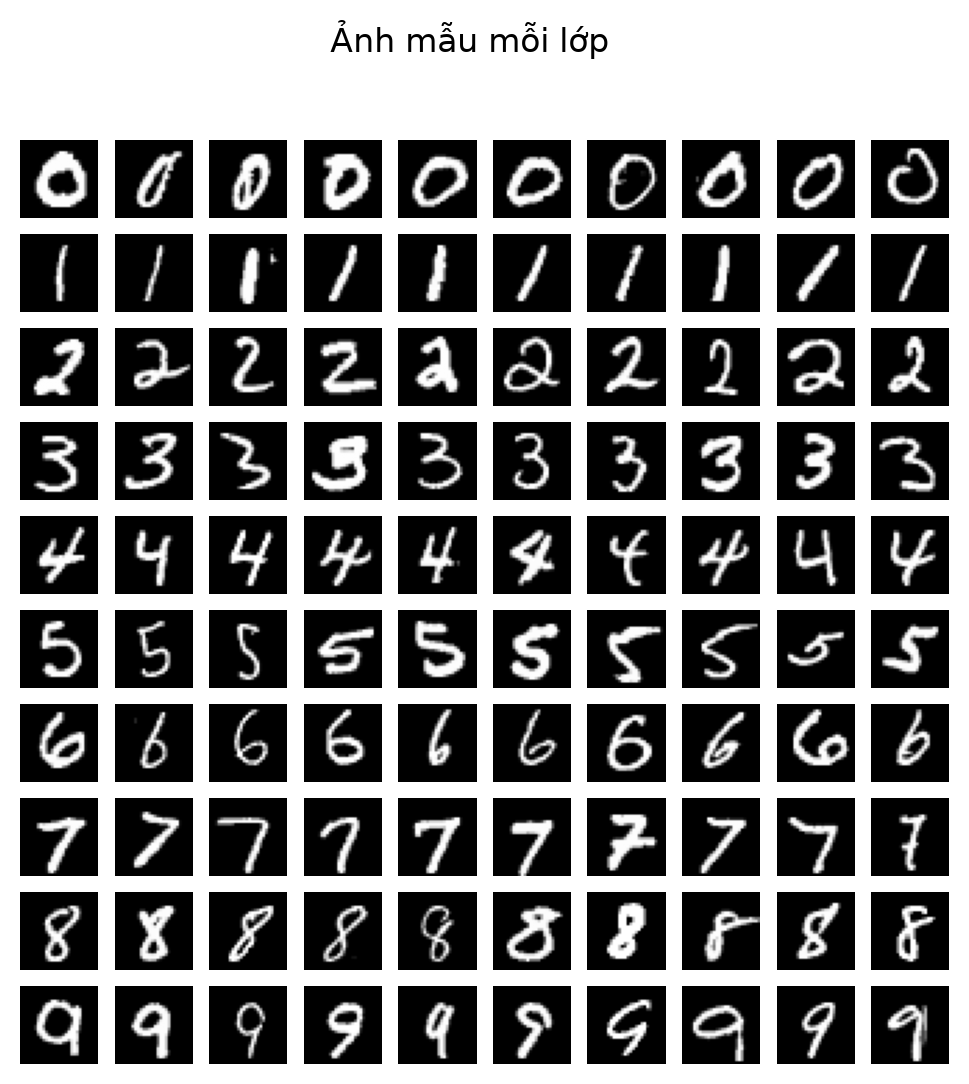
\includegraphics[width=\linewidth]{figures/eda_samples.png}
    \subcaption{Ảnh mẫu (mỗi hàng một lớp)}
  \end{minipage}\hfill
  \begin{minipage}[b]{0.62\linewidth}\centering
    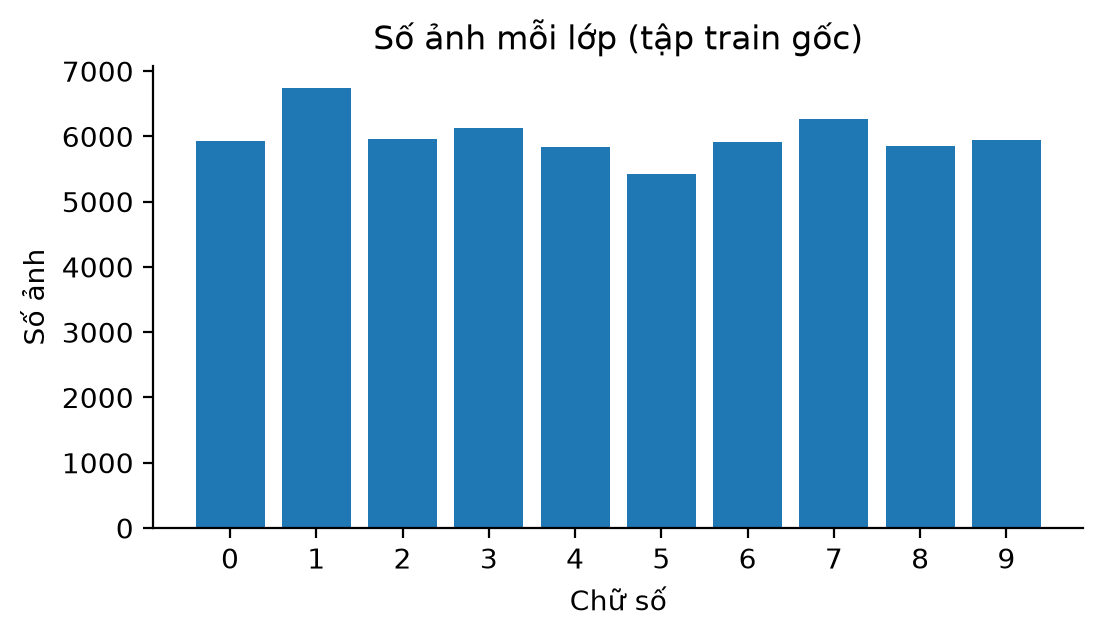
\includegraphics[width=\linewidth]{figures/eda_class_counts.png}
    \subcaption{Số ảnh mỗi lớp trong 60.000 ảnh huấn luyện gốc}
  \end{minipage}
  \caption{(a) Mười ảnh ngẫu nhiên của mỗi chữ số trong tập huấn luyện. (b) Phân bố lớp: ít nhất 5.421 ảnh (số 5), nhiều nhất 6.742 ảnh (số 1).}
  \label{fig:eda1}
\end{figure}

\textbf{Độ đa dạng và phân bố lớp.} Hình~\ref{fig:eda1}a cho thấy nét viết trong cùng lớp khác nhau đáng kể về độ nghiêng, độ dày và kiểu viết (số 4 nét hở hoặc kín, số 7 có hoặc không gạch ngang); các cặp dễ nhầm là 4--9, 3--5--8 và 7--1. Theo Hình~\ref{fig:eda1}b, số mẫu mỗi lớp dao động từ 5.421 (số 5) đến 6.742 (số 1), tỉ lệ lớn nhất/nhỏ nhất là 1,24. Dữ liệu khá cân bằng nên accuracy vẫn có ý nghĩa; nhóm báo cáo thêm precision, recall và F1 macro để mọi lớp có trọng số như nhau.

\begin{figure}[H]
  \centering
  \begin{minipage}{\linewidth}\centering
    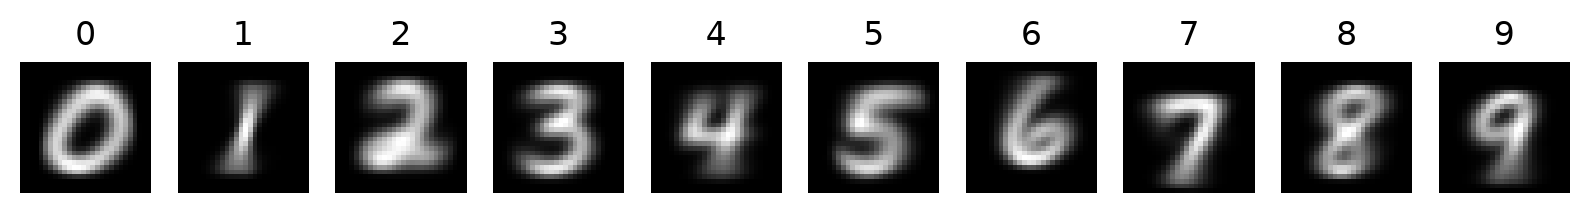
\includegraphics[width=0.92\linewidth]{figures/eda_mean_images.png}
    \subcaption{Ảnh trung bình của từng lớp}
  \end{minipage}\\[4pt]
  \begin{minipage}{\linewidth}\centering
    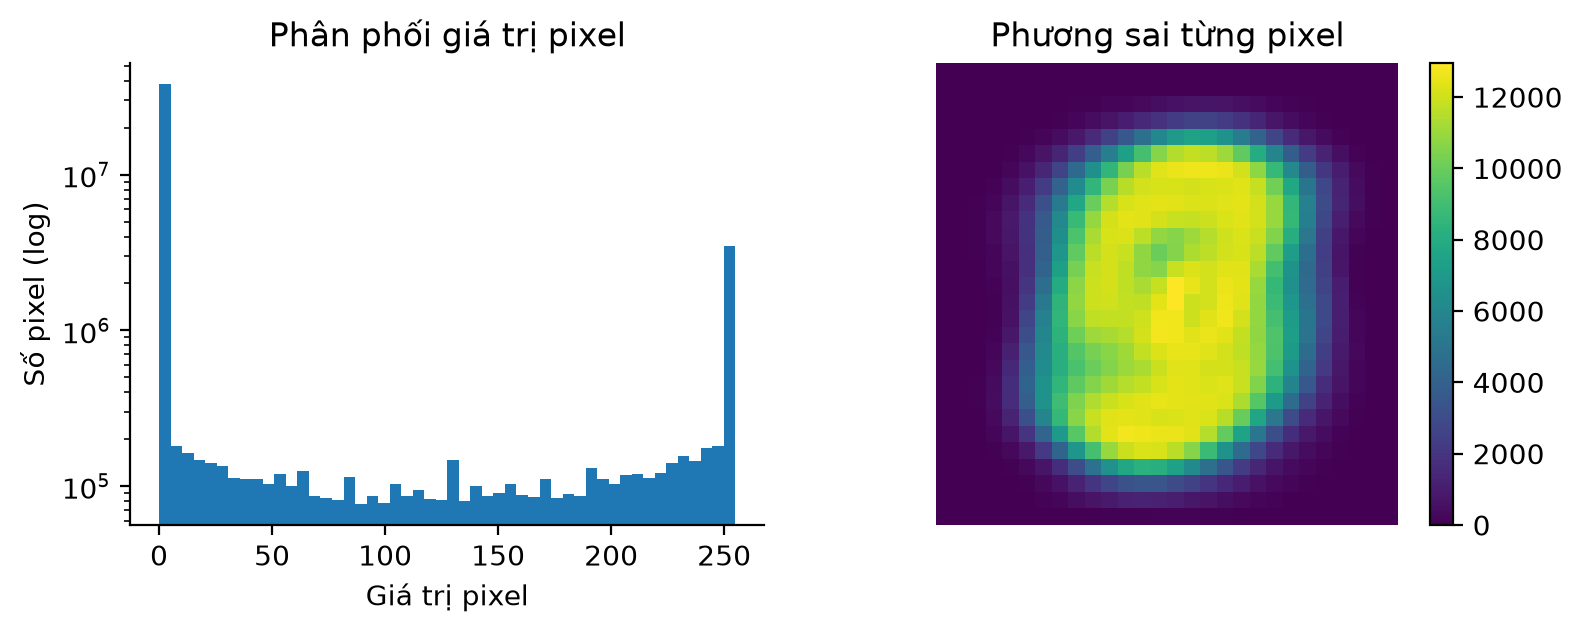
\includegraphics[width=0.8\linewidth]{figures/eda_pixels.png}
    \subcaption{Histogram giá trị pixel (trục tung thang log) và phương sai của từng pixel}
  \end{minipage}
  \caption{Thống kê pixel trên 60.000 ảnh huấn luyện gốc (giá trị 0--255).}
  \label{fig:meanstd}
\end{figure}

\textbf{Giá trị pixel.} Ảnh rất thưa: 80,9\% giá trị pixel bằng 0, và histogram (Hình~\ref{fig:meanstd}b) có hai đỉnh rõ tại 0 (nền) và 255 (lõi nét), các giá trị trung gian chỉ xuất hiện ở viền nét do khử răng cưa. Trung bình mỗi ảnh có khoảng 150 pixel nét; số 1 ít nhất (85,8) và số 0 nhiều nhất (192,0). Bản đồ phương sai cho thấy thông tin tập trung ở vùng giữa ảnh; 67/784 pixel ở viền có phương sai bằng 0, tức luôn bằng 0 trên toàn tập huấn luyện, nên không mang thông tin phân lớp. Ảnh trung bình của từng lớp (Hình~\ref{fig:meanstd}a) đã phân biệt được bằng mắt, gợi ý rằng ngay cả bộ phân lớp tuyến tính cũng có thể đạt kết quả khá; các cặp có ảnh trung bình gần nhau như 4--9 và 3--5--8 được dự báo là dễ nhầm.

\subsection{Tiền xử lý}
\label{sec:prep}
\textbf{Làm phẳng.} Lớp \code{Flattener} biến mỗi ảnh thành vector $\mathbf{x}\in\R^{784}$ theo thứ tự hàng (pixel $(i,j)$ ở vị trí $28i+j$) và ép sang \code{float32} để tránh tràn số khi tính trên \code{uint8}.

\textbf{Chuẩn hoá.} Cả bốn mô hình dùng chung chuẩn hoá min-max $x'=x/255\in[0,1]$. Cách này giữ đặc trưng không âm (điều kiện của Multinomial Na\"{\i}ve Bayes), không cần ước lượng tham số từ dữ liệu nên không có nguy cơ rò rỉ thông tin từ validation/test, và đưa đầu vào về thang đo phù hợp với khởi tạo He của MLP. Với các mô hình softmax, nhãn được mã hoá one-hot.

\subsection{Chia tập}
Tập kiểm thử (10.000 ảnh) được giữ nguyên và chỉ dùng một lần cho đánh giá cuối. Từ 60.000 ảnh huấn luyện, lớp \code{StratifiedSplitter} tách 10\% (6.000 ảnh) làm validation theo cách \emph{phân tầng}: lớp $c$ đóng góp $n_c/10$ mẫu. Vì các giá trị này không nguyên, nhóm dùng phương pháp \emph{phần dư lớn nhất}: làm tròn xuống (tổng 5.996) rồi cộng 1 mẫu cho 4 lớp có phần thập phân lớn nhất (lớp 9, 2, 6, 7), bảo đảm tổng đúng 6.000. Hạt giống cố định (\code{seed = 42}) giúp mọi thành viên dùng chung một cách chia. Validation dùng để chọn siêu tham số và dừng sớm.

\begin{table}[H]
  \centering
  \caption{Ba tập sau tiền xử lý (giá trị pixel đã chia 255).}
  \label{tab:split}
  \small
  \begin{tabular}{lrccc}
    \toprule
    Tập & Số mẫu & Số mẫu mỗi lớp (ít nhất -- nhiều nhất) & Trung bình & Độ lệch chuẩn \\
    \midrule
    Train      & 54.000 & 4.879 (số 5) -- 6.068 (số 1) & 0,131 & 0,308 \\
    Validation & 6.000  & 542 (số 5) -- 674 (số 1)     & 0,131 & 0,308 \\
    Test       & 10.000 & 892 (số 5) -- 1.135 (số 1)   & 0,133 & 0,311 \\
    \bottomrule
  \end{tabular}
\end{table}

Thống kê ba tập rất gần nhau, xác nhận việc chia không làm lệch phân bố. Toàn bộ pipeline được đóng gói trong lớp \code{MNISTPreprocessor}, gọi qua hàm \code{load\_and\_prepare} trong notebook.